\subsection{Cardinality and Infinite Sets}

% **Role:** rigorous language of real and complex analysis.
%
% Countable/uncountable sets, Cantor arguments, cardinal comparison, countable operations.


Cardinality counts sets by matching them with other sets, using the earlier language of functions, power sets, and bijections.
The foundational prerequisites collect same cardinality, finite/countable vocabulary, Cantor's theorem, Schroeder--Bernstein, and basic cardinal arithmetic; this subsection develops countability, diagonal arguments, finite-set summation, and the continuum.

\begin{proposition} \label{prop:finite-cardinality-well-defined} \hlt{Finite Cardinality is Well Defined}\\
If $A\sim_{\#}J_m$ and $A\sim_{\#}J_n$, then $m=n$. Thus $\#A=n$ is well defined for finite sets.
\begin{proof}
By transitivity of $\sim_{\#}$, it suffices to prove $J_m\sim_{\#}J_n\Rightarrow m=n$. Induct on $m$.\\
For $m=0$, only $J_0=\emptyset$ is bijective to $J_0$.\\
If $m,n\geq1$ and $f:J_m\to J_n$ is bijective, remove $m$ and its partner $f(m)$. The remaining sets are bijective and relabel as $J_{m-1}$ and $J_{n-1}$, so induction gives $m-1=n-1$, hence $m=n$.\\
\hlt{Structural Commentary}: Finite counting is invariant under bijection.\\
\hlt{Key Insight}: Remove one matched element and count down.
\end{proof}
\end{proposition}

\begin{definition} \label{def:finite-set-summation} \hlt{Summation over a Finite Set}\\
Let $X$ be a finite set with $\#X=n$, and let $f:X\to\C$.\\
Choose any bijection $g:J_n\to X$, where $J_n=\{1,\ldots,n\}$, and set $\sum\limits_{x\in X}f(x)\defeq\sum_{i=1}^{n}f(g(i))$.\\
When $X=\emptyset$, this is the empty sum $0$.\\
\hlt{Key Insight}: Proposition \ref{prop:finite-set-summation-laws} shows that the value is independent of the chosen bijection.
\end{definition}

\begin{proposition} \label{prop:finite-set-summation-laws} \hlt{Finite Set Summation Laws}\\
Let $X,Y$ be finite sets.
\begin{enumerate}[label=(\roman*)]
\setlength{\itemsep}{0pt}
\item \hlt{Well-definedness}: different bijections $J_{\#X}\to X$ give the same value in Definition \ref{def:finite-set-summation}.
\item \hlt{Substitution}: if $h:Y\to X$ is a bijection and $f:X\to\C$, then $\sum\limits_{x\in X}f(x)=\sum\limits_{y\in Y}f(h(y))$.
\item \hlt{Linearity}: for $f,g:X\to\C$ and $c\in\C$, $\sum\limits_{x\in X}(f(x)+g(x))=\sum\limits_{x\in X}f(x)+\sum\limits_{x\in X}g(x)$ and $\sum\limits_{x\in X}cf(x)=c\sum\limits_{x\in X}f(x)$.
\item \hlt{Disjoint unions}: if $X\cap Y=\emptyset$ and $f:X\cup Y\to\C$, then $\sum\limits_{z\in X\cup Y}f(z)=\sum\limits_{x\in X}f(x)+\sum\limits_{y\in Y}f(y)$.
\item \hlt{Finite Fubini}: if $f:X\times Y\to\C$, then $\sum\limits_{x\in X}\sum\limits_{y\in Y}f(x,y)=\sum\limits_{(x,y)\in X\times Y}f(x,y)=\sum\limits_{y\in Y}\sum\limits_{x\in X}f(x,y)$.
\end{enumerate}
\begin{proof}
\begin{enumerate}[label=(\roman*)]
\setlength{\itemsep}{0pt}
\item For $f:X\to\C$, let $n=\#X$ and let $g,k:J_n\to X$ be bijections. Induct on $n$. The case $n=0$ is empty. If $n\geq1$, let $j\in J_n$ satisfy $k(j)=g(n)$. Removing $n$ from $g$ and $j$ from $k$ gives bijections onto $X\setminus\{g(n)\}$; after relabeling by $J_{n-1}$, the induction hypothesis makes the remaining sums equal. Adding the common last term $f(g(n))=f(k(j))$ gives equality of the two sums.
\item Let $g:J_{\#Y}\to Y$ be a bijection. Then $h\circ g:J_{\#Y}\to X$ is a bijection, so $\#Y=\#X$ by Proposition \ref{prop:finite-cardinality-well-defined}.\\
Hence, by (i) and Definition \ref{def:finite-set-summation}, $\sum\limits_{x\in X}f(x)=\sum\limits_{i=1}^{\#Y}f(h(g(i)))=\sum\limits_{y\in Y}f(h(y))$.
\item Choose a bijection $\gamma:J_{\#X}\to X$.\\
Proposition \ref{prop:finite-sum-basic-laws} gives $\sum\limits_{x\in X}(f(x)+g(x)) =\sum\limits_{x\in X}f(x)+\sum\limits_{x\in X}g(x)$ and $\sum\limits_{x\in X}cf(x)=c\sum\limits_{x\in X}f(x)$
\item Let $\alpha:J_{\#X}\to X$ and $\beta:J_{\#Y}\to Y$ be bijections, and enumerate $X\cup Y$ by listing $\alpha$ first and then $\beta$. Since $X\cap Y=\emptyset$, this is a bijection, and Proposition \ref{prop:finite-sum-basic-laws} gives $\sum\limits_{z\in X\cup Y}f(z)=\sum\limits_{x\in X}f(x)+\sum\limits_{y\in Y}f(y)$.
\item Let $\alpha:J_{\#X}\to X$ and $\beta:J_{\#Y}\to Y$ be bijections.\\
The maps $\ell((i-1)\#Y+j)=(\alpha(i),\beta(j))$ and $r((j-1)\#X+i)=(\alpha(i),\beta(j))$ for $i\in J_{\#X}$ and $j\in J_{\#Y}$ give the two lexicographic bijections $J_{(\#X)(\#Y)}\to X\times Y$.\\
Applying Definition \ref{def:finite-set-summation}, Proposition \ref{prop:finite-sum-basic-laws}, and (i) yields $\sum\limits_{x\in X}\sum\limits_{y\in Y}f(x,y) =\sum\limits_{(x,y)\in X\times Y}f(x,y) =\sum\limits_{y\in Y}\sum\limits_{x\in X}f(x,y)$.
\end{enumerate}
\hlt{Structural Commentary}: A finite set sum is an order-free finite sum.\\
\hlt{Key Insight}: Bijections are bookkeeping devices; the value does not depend on the bookkeeping order.
\end{proof}
\end{proposition}

\begin{definition} \label{def:sequence-as-enumeration} \hlt{Sequences as Enumerations}\\
A \hlt{sequence} in set $A$ is $x:\N\to A$, written $(x_n)$, where $x_n\defeq x(n)$. Terms of sequence need not be distinct.\\
If $A$ is countable, then its elements can be arranged as a sequence with distinct terms. Conversely, a sequence whose terms are distinct and whose range is $A$ gives a bijection $\N\to A$.
\end{definition}

\begin{example} \label{ex:integers-are-countable} \hlt{The Integers Are Countable}\\
The set $\Z$ is countable. One explicit enumeration is given by
\begin{align}
f(n)=
\begin{cases}
\frac{n}{2}, & n \text{ even},\\[2mm]
-\frac{n-1}{2}, & n \text{ odd},
\end{cases}
\qquad n\in\N. \nonumber
\end{align}
This lists $\Z$ as $0,1,-1,2,-2,3,-3,\ldots$.
\end{example}

\begin{theorem} \label{thm:infinite-subset-of-countable-is-countable} \hlt{Infinite Subsets of Countable Sets}\\
Every infinite subset of a countable set is countable.
\begin{proof}
Let $E\subseteq A$ be infinite, and enumerate $A$ by distinct terms $(x_n)$. Let $n_1<n_2<\cdots$ be exactly the indices for which $x_{n_k}\in E$, listed in increasing order. Then $k\mapsto x_{n_k}$ is a bijection from $\N$ onto $E$.\\
\hlt{Structural Commentary}: The proof keeps only the entries of the original enumeration that land in $E$.\\
\hlt{Key Insight}: An infinite subset of an enumeration inherits an enumeration by first appearances.
\end{proof}
\end{theorem}

\begin{proposition} \label{prop:subsets-and-images-at-most-countable} \hlt{Subsets and Images of At Most Countable Sets}\\
Let $A$ be at most countable.
\begin{enumerate}[label=(\roman*)]
\setlength{\itemsep}{0pt}
\item If $B\subseteq A$, then $B$ is at most countable.
\item If $f:A\to Y$ is a function, then $f(A)$ is at most countable.
\end{enumerate}
\begin{proof}
If $A$ is finite, both claims are immediate. Otherwise write $A=\{a_n:n\in\N\}$ with the $a_n$ distinct.
\begin{enumerate}[label=(\roman*)]
\setlength{\itemsep}{0pt}
\item If $B$ is infinite, let $I_B\defeq\{n:a_n\in B\}=\{n_1<n_2<\cdots\}$.\\
Then $k\mapsto a_{n_k}$ bijects $\N$ onto $B$; the finite case is trivial.
\item Let $I\defeq\{n:f(a_n)\notin\{f(a_m):m<n\}\}$. By (i), $I$ is at most countable, $n\mapsto f(a_n)$ bijects $I$ onto $f(A)$.
\end{enumerate}
\hlt{Structural Commentary}: Subsets select indices; images select first appearances.\\
\hlt{Key Insight}: Subsets and images preserve at-most-countability.
\end{proof}
\end{proposition}

\begin{figure}[H]
  \centering
  \begin{tikzpicture}[
  >=Stealth,
  every node/.style={font=\small},
  entry/.style={draw=gray!55, fill=gray!5, rounded corners=1pt, minimum width=0.62cm, minimum height=0.40cm},
  active/.style={draw=orange!60!black, fill=orange!10},
  scan/.style={->, blue!70!black, line width=0.7pt},
  guide/.style={orange!75!black, line width=0.65pt},
  output/.style={draw=gray!55, fill=gray!5, rounded corners=1pt, inner xsep=5pt, inner ysep=4pt}
]
  \draw[guide] (1.70,-0.65) -- (0.85,-1.30);
  \draw[guide] (2.55,-0.65) -- (0.85,-1.95);
  \draw[guide] (3.40,-0.65) -- (0.85,-2.60);

  \foreach \row/\name in {1/E_1,2/E_2,3/E_3,4/E_4} {
    \node[anchor=east] at (0,-0.65*\row) {$\name$};
    \foreach \col in {1,...,5} {
      \node[entry] (x-\row-\col) at (0.85*\col,-0.65*\row) {$x_{\row\col}$};
    }
    \node[anchor=west, gray!65] at (4.55,-0.65*\row) {$\cdots$};
  }

  \foreach \row/\col in {1/1,1/2,2/1,1/3,2/2,3/1,1/4,2/3,3/2,4/1} {
    \node[entry, active] at (0.85*\col,-0.65*\row) {$x_{\row\col}$};
  }

  \node[output, anchor=west] (list) at (5.25,-1.45)
    {$x_{11},\,x_{12},\,x_{21},\,x_{13},\,x_{22},\,x_{31},\,x_{14},\,\cdots$};
  \draw[scan] (4.55,-1.45) -- (list.west);
\end{tikzpicture}

  \caption{Diagonal scan of countable rows into one sequence, skipping repeats.}
  \label{fig:countable-union-diagonal-scan}
\end{figure}

\begin{theorem} \label{thm:countable-union-of-countable-sets}\label{thm:cardinality-main-results-source-todo} \hlt{Countable Union of Countable Sets}\\
Let $(E_n)$ be a sequence of countable sets and put $S\defeq\bigcup\limits_{n=1}^{\infty}E_n$. Then $S$ is countable.
\begin{proof}
Enumerate each $E_n$ as $(x_{nk})_{k\in\N}$.\\
Reading the array $(x_{nk})$ by diagonals, as in Figure \ref{fig:countable-union-diagonal-scan}, gives a sequence whose image is $S$.\\
Thus $S$ is at most countable by Proposition \ref{prop:subsets-and-images-at-most-countable}.\\
Since $E_1\subseteq S$ and $E_1$ is countable, $S$ is infinite; hence $S$ is countable.\\
\hlt{Structural Commentary}: The diagonal order turns a two-indexed list into a one-indexed list.\\
\hlt{Key Insight}: Countably many countable rows can still be scanned by one sequence.
\end{proof}
\end{theorem}

\begin{corollary} \label{cor:at-most-countable-union-at-most-countable} \hlt{At Most Countable Unions}\\
If $A$ is at most countable and $B_\alpha$ is at most countable for each $\alpha\in A$, then $\bigcup\limits_{\alpha\in A}B_\alpha$ is at most countable.
\begin{proof}
Let $T\defeq\bigcup\limits_{\alpha\in A}B_\alpha$. If $T=\emptyset$, we are done. Otherwise enumerate the nonempty sets among the $B_\alpha$ as $B_{\alpha_1},B_{\alpha_2},\ldots$, repeating indices if needed, and list each $B_{\alpha_j}$ as $(b_{jk})_{k\in\N}$.\\
A diagonal scan of $(b_{jk})$ has image $T$, so Proposition \ref{prop:subsets-and-images-at-most-countable} makes $T$ at most countable.\\
\hlt{Structural Commentary}: Finite pieces cause no difficulty; they can be embedded into countable rows.\\
\hlt{Key Insight}: At most countable indexing $+$ at most countable indexed sets gives at most countable total set.
\end{proof}
\end{corollary}

\begin{theorem} \label{thm:finite-tuples-over-countable-set-countable} \hlt{Finite Tuples over a Countable Set}\\
Let $A$ be countable. For each fixed $n\in\N$, the set of all $n$-tuples $(a_1,\ldots,a_n)$ with $a_k\in A$ is countable.
\begin{proof} Let $B_n\defeq \{(a_1,\ldots,a_n): a_k\in A\}$, $B_1=A$. If $B_{n-1}$ is countable, $B_n=\bigcup\limits_{b\in B_{n-1}}\{(b,a):a\in A\}$, each set $\{(b,a):a\in A\}$ is equivalent to $A$. Hence $B_n$ is countable by Theorem \ref{thm:countable-union-of-countable-sets}.\\
\hlt{Structural Commentary}: Build an $n$-tuple by appending one coordinate to an $(n-1)$-tuple.\\
\hlt{Key Insight}: Induction plus countable unions controls finite products.
\end{proof}
\end{theorem}

\begin{figure}[H]
  \centering
  \begin{tikzpicture}[
  x=0.82cm,
  y=0.82cm,
  >=Stealth,
  every node/.style={font=\small},
  point/.style={circle, fill=black, inner sep=1.25pt},
  active/.style={circle, draw=orange!60!black, fill=orange!12, line width=0.55pt, inner sep=2.2pt},
  guide/.style={orange!75!black, line width=0.65pt},
  scan/.style={->, blue!70!black, line width=0.7pt},
  output/.style={draw=gray!55, fill=gray!5, rounded corners=1pt, inner xsep=5pt, inner ysep=4pt}
]
  \foreach \i in {1,...,5} {
    \node[anchor=east] at (0,-0.42*\i) {$\i$};
    \node[anchor=south] at (0.47*\i,-0.1) {$\i$};
  }
  \node[anchor=south] at (2.65,-0.1) {$\cdots$};

  \draw[guide] (0.94,-0.42) -- (0.47,-0.84);
  \draw[guide] (1.41,-0.42) -- (0.47,-1.26);
  \draw[guide] (1.88,-0.42) -- (0.47,-1.68);

  \foreach \row in {1,...,5} {
    \foreach \col in {1,...,5} {
      \node[point] at (0.47*\col,-0.42*\row) {};
    }
  }

  \foreach \row/\col in {1/1,1/2,2/1,1/3,2/2,3/1,1/4,2/3,3/2,4/1} {
    \node[active] at (0.47*\col,-0.42*\row) {};
  }

  \node[output, anchor=west] (list) at (3.10,-1.05)
    {$(1,1),\,(1,2),\,(2,1),\,(1,3),\,(2,2),\,(3,1),\,\cdots$};
  \draw[scan] (2.70,-1.05) -- (list.west);
\end{tikzpicture}

  \caption{Diagonal enumeration of $\N\times\N$ by finite $i+j$ diagonals.}
  \label{fig:countable-diagonal-enumeration}
\end{figure}

\begin{corollary} \label{cor:countable-cartesian-products} \hlt{Countable Cartesian Products}\\
If $A,B$ are at most countable, then $A\times B$ is at most countable.\\
If $A,B$ are countable and nonempty, then $A\times B$ is countable. Hence $\N\times\N$ is countable.
\begin{proof}
For $a\in A$, $\{a\}\times B\sim B$, and $A\times B=\bigcup\limits_{a\in A}\bigl(\{a\}\times B\bigr)$, thus $A\times B$ at most countable (Corollary \ref{cor:at-most-countable-union-at-most-countable}). If $A,B$ are countable and $b_0\in B$, then $a\mapsto(a,b_0)$ injects $A$ into $A\times B$, so $A\times B$ is infinite; hence it is countable.\\
\hlt{Structural Commentary}: A product is a countable union of countable slices.\\
\hlt{Key Insight}: Two countable coordinates can still be scanned by one sequence.
\end{proof}
\end{corollary}

\begin{corollary} \label{cor:rationals-countable} \hlt{The Rationals Are Countable}\\
The set $\Q$ is countable.
\begin{proof}
Let $D\defeq\{(a,b)\in\Z\times\Z:a\neq0\}$ and $\pi:D\to\Q$ by $\pi(a,b)=b/a$.\\
Since $\Z$ is countable, Corollary \ref{cor:countable-cartesian-products} and Proposition \ref{prop:subsets-and-images-at-most-countable} make $D$ at most countable. Since $\pi(D)=\Q$, Proposition \ref{prop:subsets-and-images-at-most-countable} makes $\Q$ at most countable. As $\Z\subseteq\Q$, it is countable.\\
\hlt{Structural Commentary}: Repeated fractions only add repetitions to the list.\\
\hlt{Key Insight}: Countable pairs produce countably many rational values.
\end{proof}
\end{corollary}

\begin{figure}[H]
  \centering
  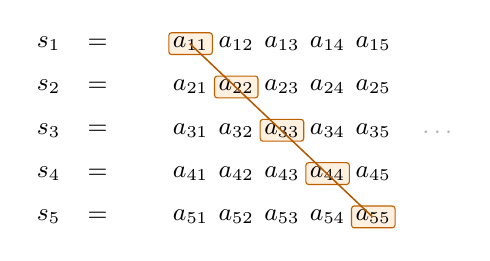
\begin{tikzpicture}[
  every node/.style={font=\small},
  digit/.style={font=\small},
  diagonal/.style={draw=orange!75!black, fill=orange!12, rounded corners=1pt, inner sep=1.5pt},
  guide/.style={orange!70!black, line width=0.55pt}
]
  \foreach \row/\name in {1/s_1,2/s_2,3/s_3,4/s_4,5/s_5} {
    \node[anchor=east] at (0,-0.55*\row) {$\name$};
    \node at (0.35,-0.55*\row) {$=$};
  }

  \foreach \row in {1,...,5} {
    \foreach \col in {1,...,5} {
      \node[digit] at (0.95+0.58*\col,-0.55*\row) {$a_{\row\col}$};
    }
  }

  \foreach \row in {1,...,5} {
    \node[diagonal] at (0.95+0.58*\row,-0.55*\row) {$a_{\row\row}$};
  }
  \draw[guide] (1.52,-0.55) -- (3.84,-2.75);

  \node[anchor=west, gray!60] at (4.35,-1.68) {$\cdots$};
\end{tikzpicture}

  \caption{Cantor diagonalization: $s(n)=1-a_{nn}$ differs from row $s_n$ at position $n$.}
  \label{fig:cantor-diagonal-binary-sequences}
\end{figure}

\begin{theorem} \label{thm:binary-sequences-uncountable} \hlt{Binary Sequences Are Uncountable}\\
Let $A$ be the set of all sequences whose terms are the digits $0$ and $1$. Then $A$ is uncountable.
\begin{proof}
Suppose $A$ were countable, $A=\{s_1,s_2,\ldots\}$ with $s_n=(s_n(k))_{k\in\N}$. Define $s\in A$ by $s(k)\defeq 1-s_k(k)$.\\
Then $s(n)\neq s_n(n)$ for every $n$, so $s\neq s_n$ for all $n$. Hence $s\notin A$, a contradiction. Thus $A$ is uncountable.\\
\hlt{Structural Commentary}: The construction attacks the diagonal of a proposed enumeration.\\
\hlt{Key Insight}: A sequence can be built to escape every row of a countable list.
\end{proof}
\end{theorem}

\begin{definition} \label{def:continuum-cardinal} \hlt{Continuum Cardinal}\\
The \hlt{continuum cardinal} is $\mathfrak{c}\defeq 2^{\aleph_0}\defeq\abs{\{0,1\}^{\N}}$. Equivalently, $\mathfrak{c}=\abs{\mathcal{P}(\N)}$ via $s\mapsto\{n\in\N:s(n)=1\}$.
\end{definition}

\begin{perspective} \label{per:continuum-and-powerset-cardinality} \hlt{Continuum Cardinality}\\
Theorem \ref{thm:binary-sequences-uncountable} and Theorem \ref{thm:cantor-power-set-theorem} give $\aleph_0<\mathfrak{c}$.\\
Thus the continuum is the first cardinal jump produced by binary choice over $\N$.
\end{perspective}

\begin{method} \label{meth:cardinality-proof-patterns}\label{meth:cardinality-proof-patterns-source-todo} \hlt{Cardinality Proof Patterns}
\begin{enumerate}[label=(\roman*)]
\setlength{\itemsep}{0pt}
\item Same cardinality: construct a bijection.
\item Countable: construct a sequence whose range contains every element.
\item Uncountable: show every proposed sequence misses some element.
\item Choice/maximality: cite Principle \ref{princ:axiom-of-choice-analysis} for arbitrary simultaneous choices and Principle \ref{princ:zorns-lemma} for maximal elements in partially ordered sets.
\end{enumerate}
\hlt{Key Idea}: Use maps: bijections prove equal cardinality, enumerations $\N\to A$ prove countability, and diagonal arguments show every proposed enumeration misses an element.
\end{method}
